%UCD: Creazione artefatto

\begin{figure}
\centering
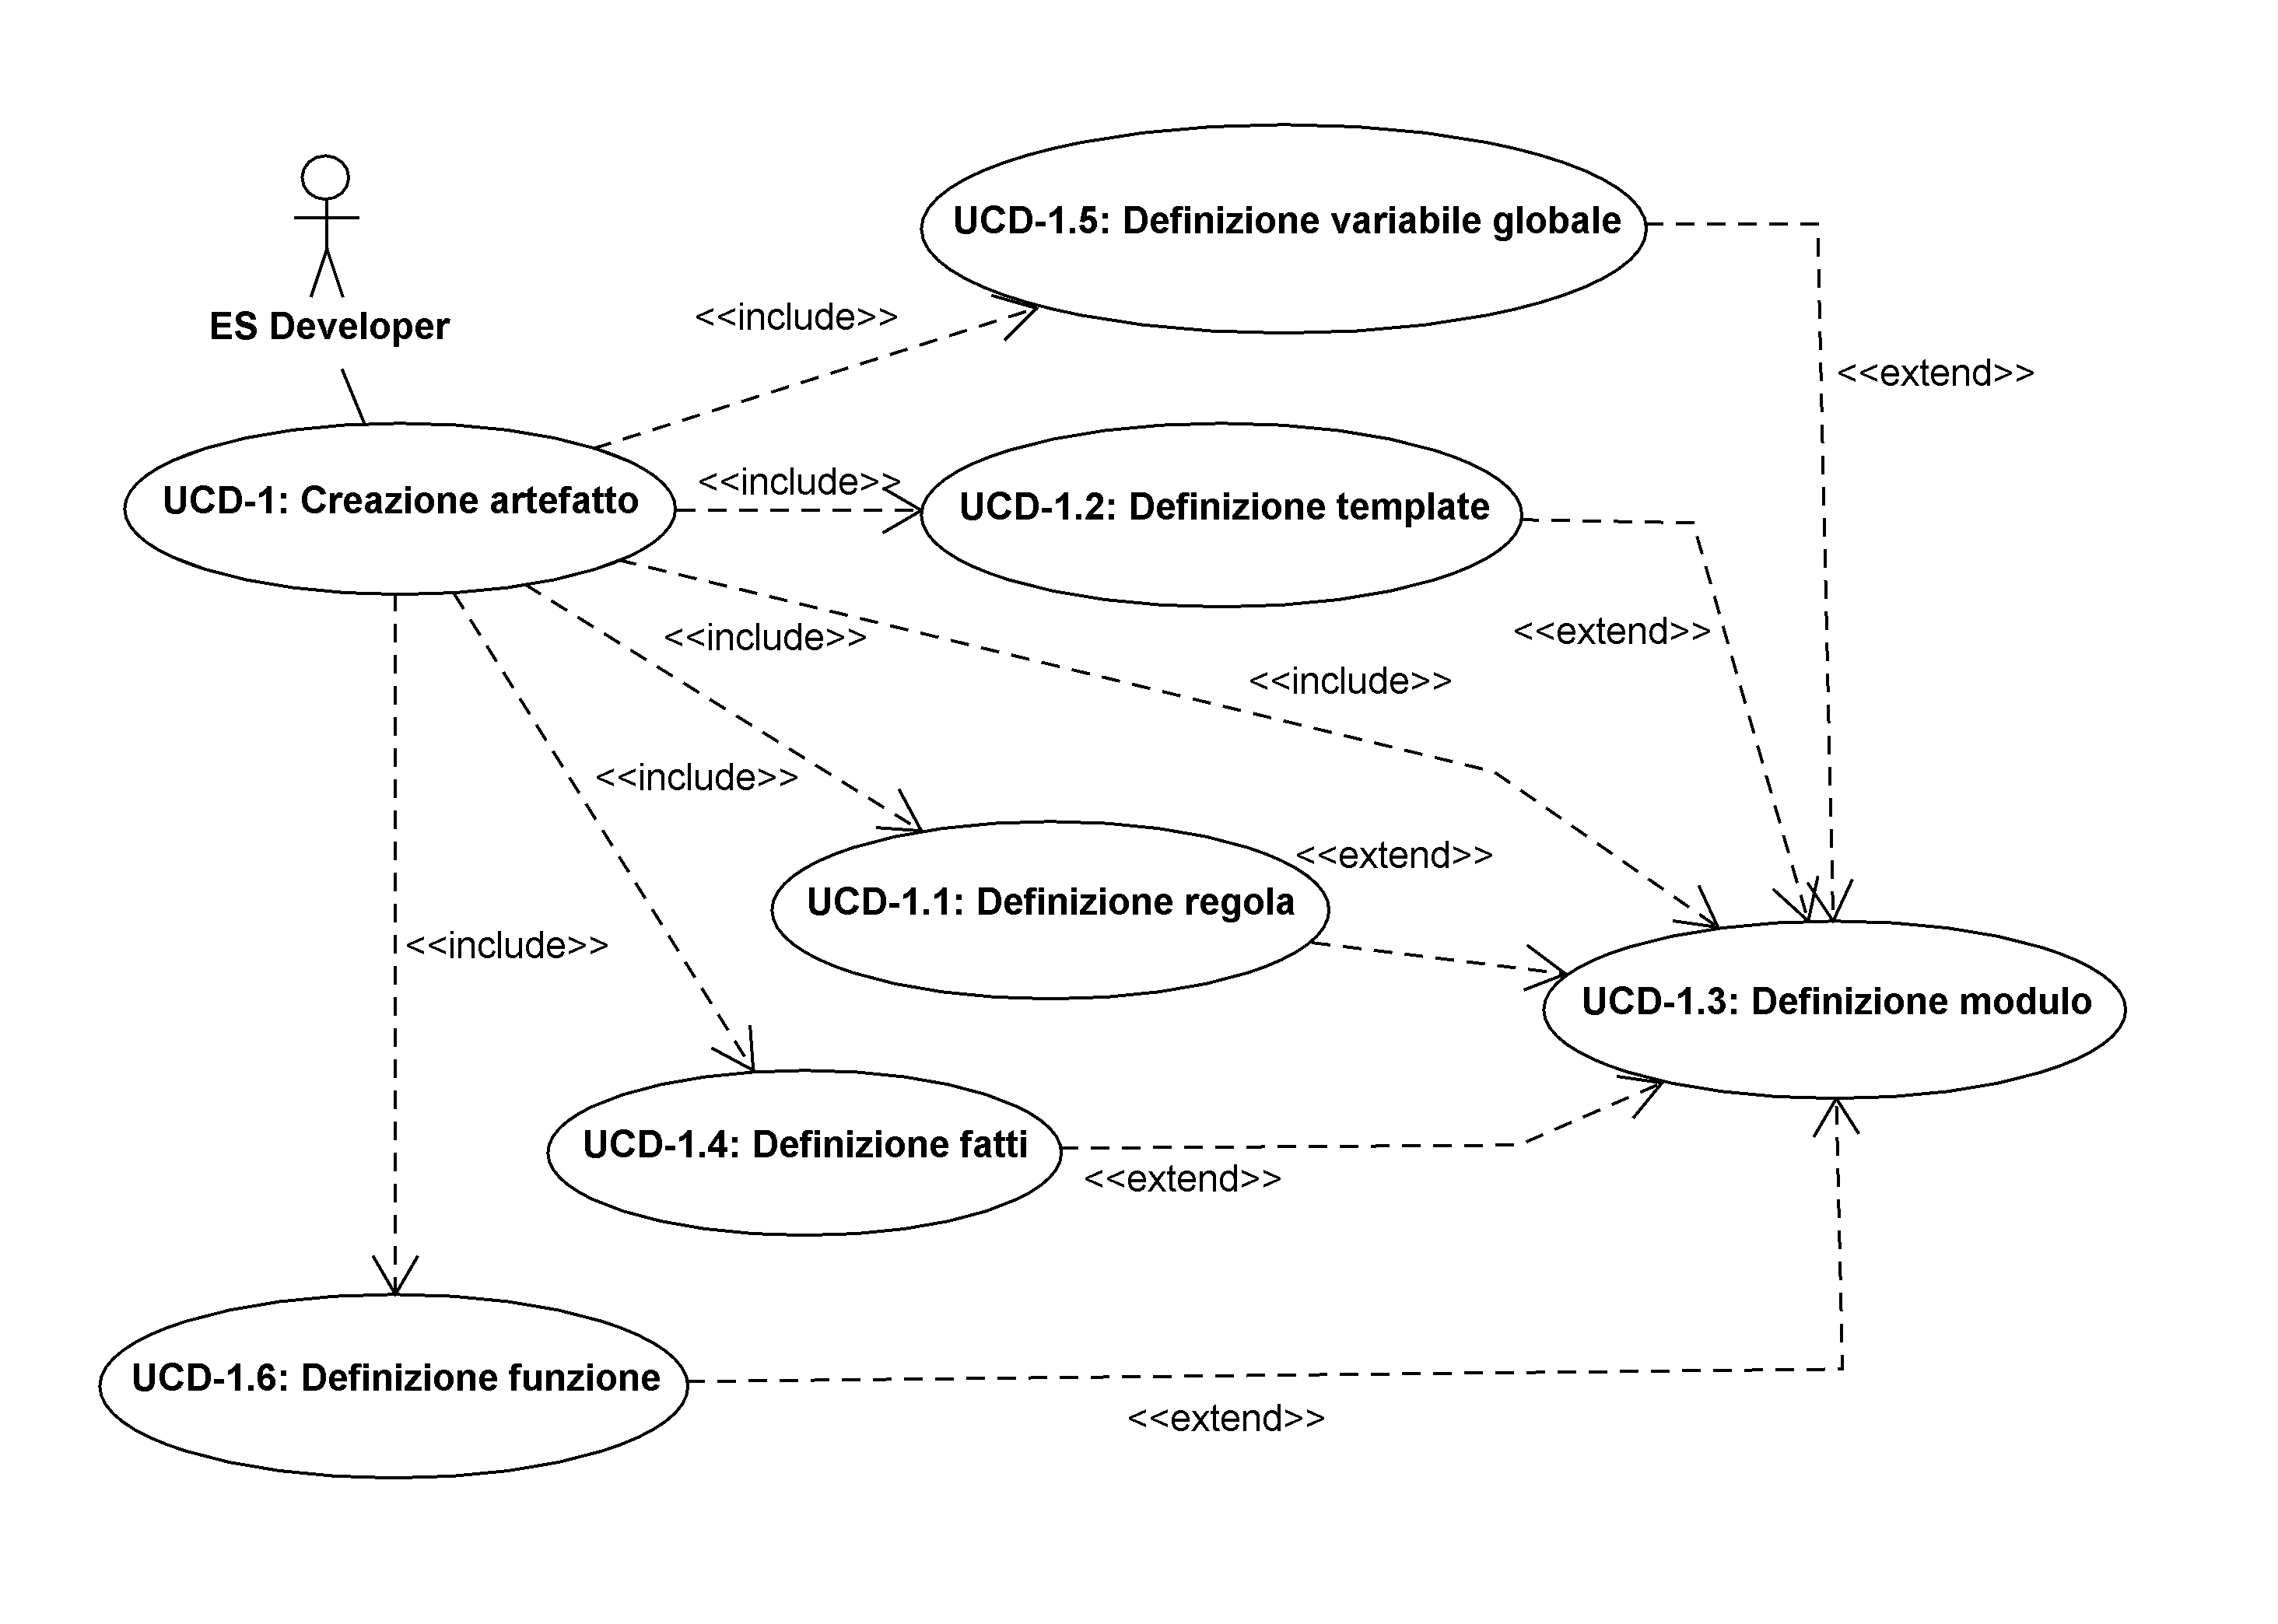
\includegraphics[width=1.1\textwidth]{Immagini/Capitolo2/UseCases/UCD-1.png}
\caption{Diagramma dei casi d'uso UCD-1}\label{fig:uc-ucd-1}
\end{figure}


\begin{itemize}
	\item \textbf{Attori:} ES Developer
	\item \textbf{Scopo e descrizione:} un ES Developer deve essere in grado di definire i costrutti necessari alla realizzazione di un artefatto.
	\item \textbf{Pre-condizioni:} il software fornisce almeno un linguaggio di specifica
	\item \textbf{Post-condizioni:} un artefatto è stato serializzato tramite il linguaggio di specifica
	\item \textbf{Flusso principale degli eventi:}
		\begin{enumerate}
			\item l'ES Developer definisce una serie di costrutti (si vedano i casi d'uso \emph{UCD-1.1}, \emph{UCD-1.2}, \emph{UCD-1.3}, \emph{UCD-1.4}, \emph{UCD-1.5}, \emph{UCD-1.6}).
			\begin{itemize}
				\item l'ES Developer può formalizzarlo in formato nativo
				\item l'ES Developer può formalizzarlo in formatto CLIPS
			\end{itemize}
			\item l'ES Consumer verifica la correttezza dell'artefatto (si veda il caso d'uso \emph{UCD-1.2}).
		\end{enumerate}
\end{itemize}


\paragraph{UCD-1.1: Definizione regola}

\begin{itemize}
	\item \textbf{Attori:} ES Developer
	\item \textbf{Scopo e descrizione:} un ES Consumer deve essere in grado di definire una regola tramite un linguaggio di specifica fornito dal sistema.
	\item \textbf{Pre-condizioni:} il software fornisce almeno un linguaggio di specifica
	\item \textbf{Post-condizioni:} la definizione di una regola è stata aggiunta ad un artefatto
	\item \textbf{Flusso principale degli eventi:}
		\begin{enumerate}
			\item l'ES Developer definisce una regola
			\begin{itemize}
				\item l'ES Developer può formalizzarla in formato nativo
				\item l'ES Developer può formalizzarla in formatto CLIPS
			\end{itemize}
		\end{enumerate}
	\item \textbf{Flusso alternativo:}
		\begin{enumerate}
			\item se l'ES Developer ha definito precedentemente un modulo, l'ES Developer può definire una regola come componente del modulo.
		\end{enumerate}
\end{itemize}


%%%%%%%%%%%%%%%% DA QUIIII %%%%%%%%%%%%%%%%%%


\paragraph{UCD-1.2: Definizione template}

\begin{itemize}
	\item \textbf{Attori:} ES Consumer
	\item \textbf{Scopo e descrizione:} l'ES Consumer deve poter eseguire un artefatto caricato nel sistema. Se l'interazione lo richiede, l'ES Consumer deve essere in grado di fornire informazioni aggiuntive, osservare l'accadimento di un evento e osservare l'output fornito dal sistema
	\item \textbf{Pre-condizioni:} il software ha correttamente caricato un artefatto ed attende istruzioni.
	\item \textbf{Post-condizioni:} il software ha correttamente eseguito le operazioni previste dall'artefatto.
	\item \textbf{Flusso principale degli eventi:}
		\begin{enumerate}
			\item l'ES Consumer richiede l'esecuzione di un artefatto
			\item il sistema esegue le operazioni previste dall'artefatto (si vedano i casi d'uso \emph{UCC-1.2.1}, \emph{UCC-1.2.3})
			\item il sistema fornisce all'ES Consumer i risultati dell'esecuzione		
		\end{enumerate}
	\item \textbf{Flusso alternativo:} 
		\begin{enumerate}
			\setcounter{enumi}{1}
			\item se un'operazione specificata nell'artefatto genera errori, il sistema notifica l'errore all'ES Consumer fornendo informazioni sulla natura del problema.
			\item il sistema ritorna nello stato iniziale
		\end{enumerate}
\end{itemize}

\paragraph{UCD-1.3: Definizione modulo}

\begin{figure}[h]
\centering
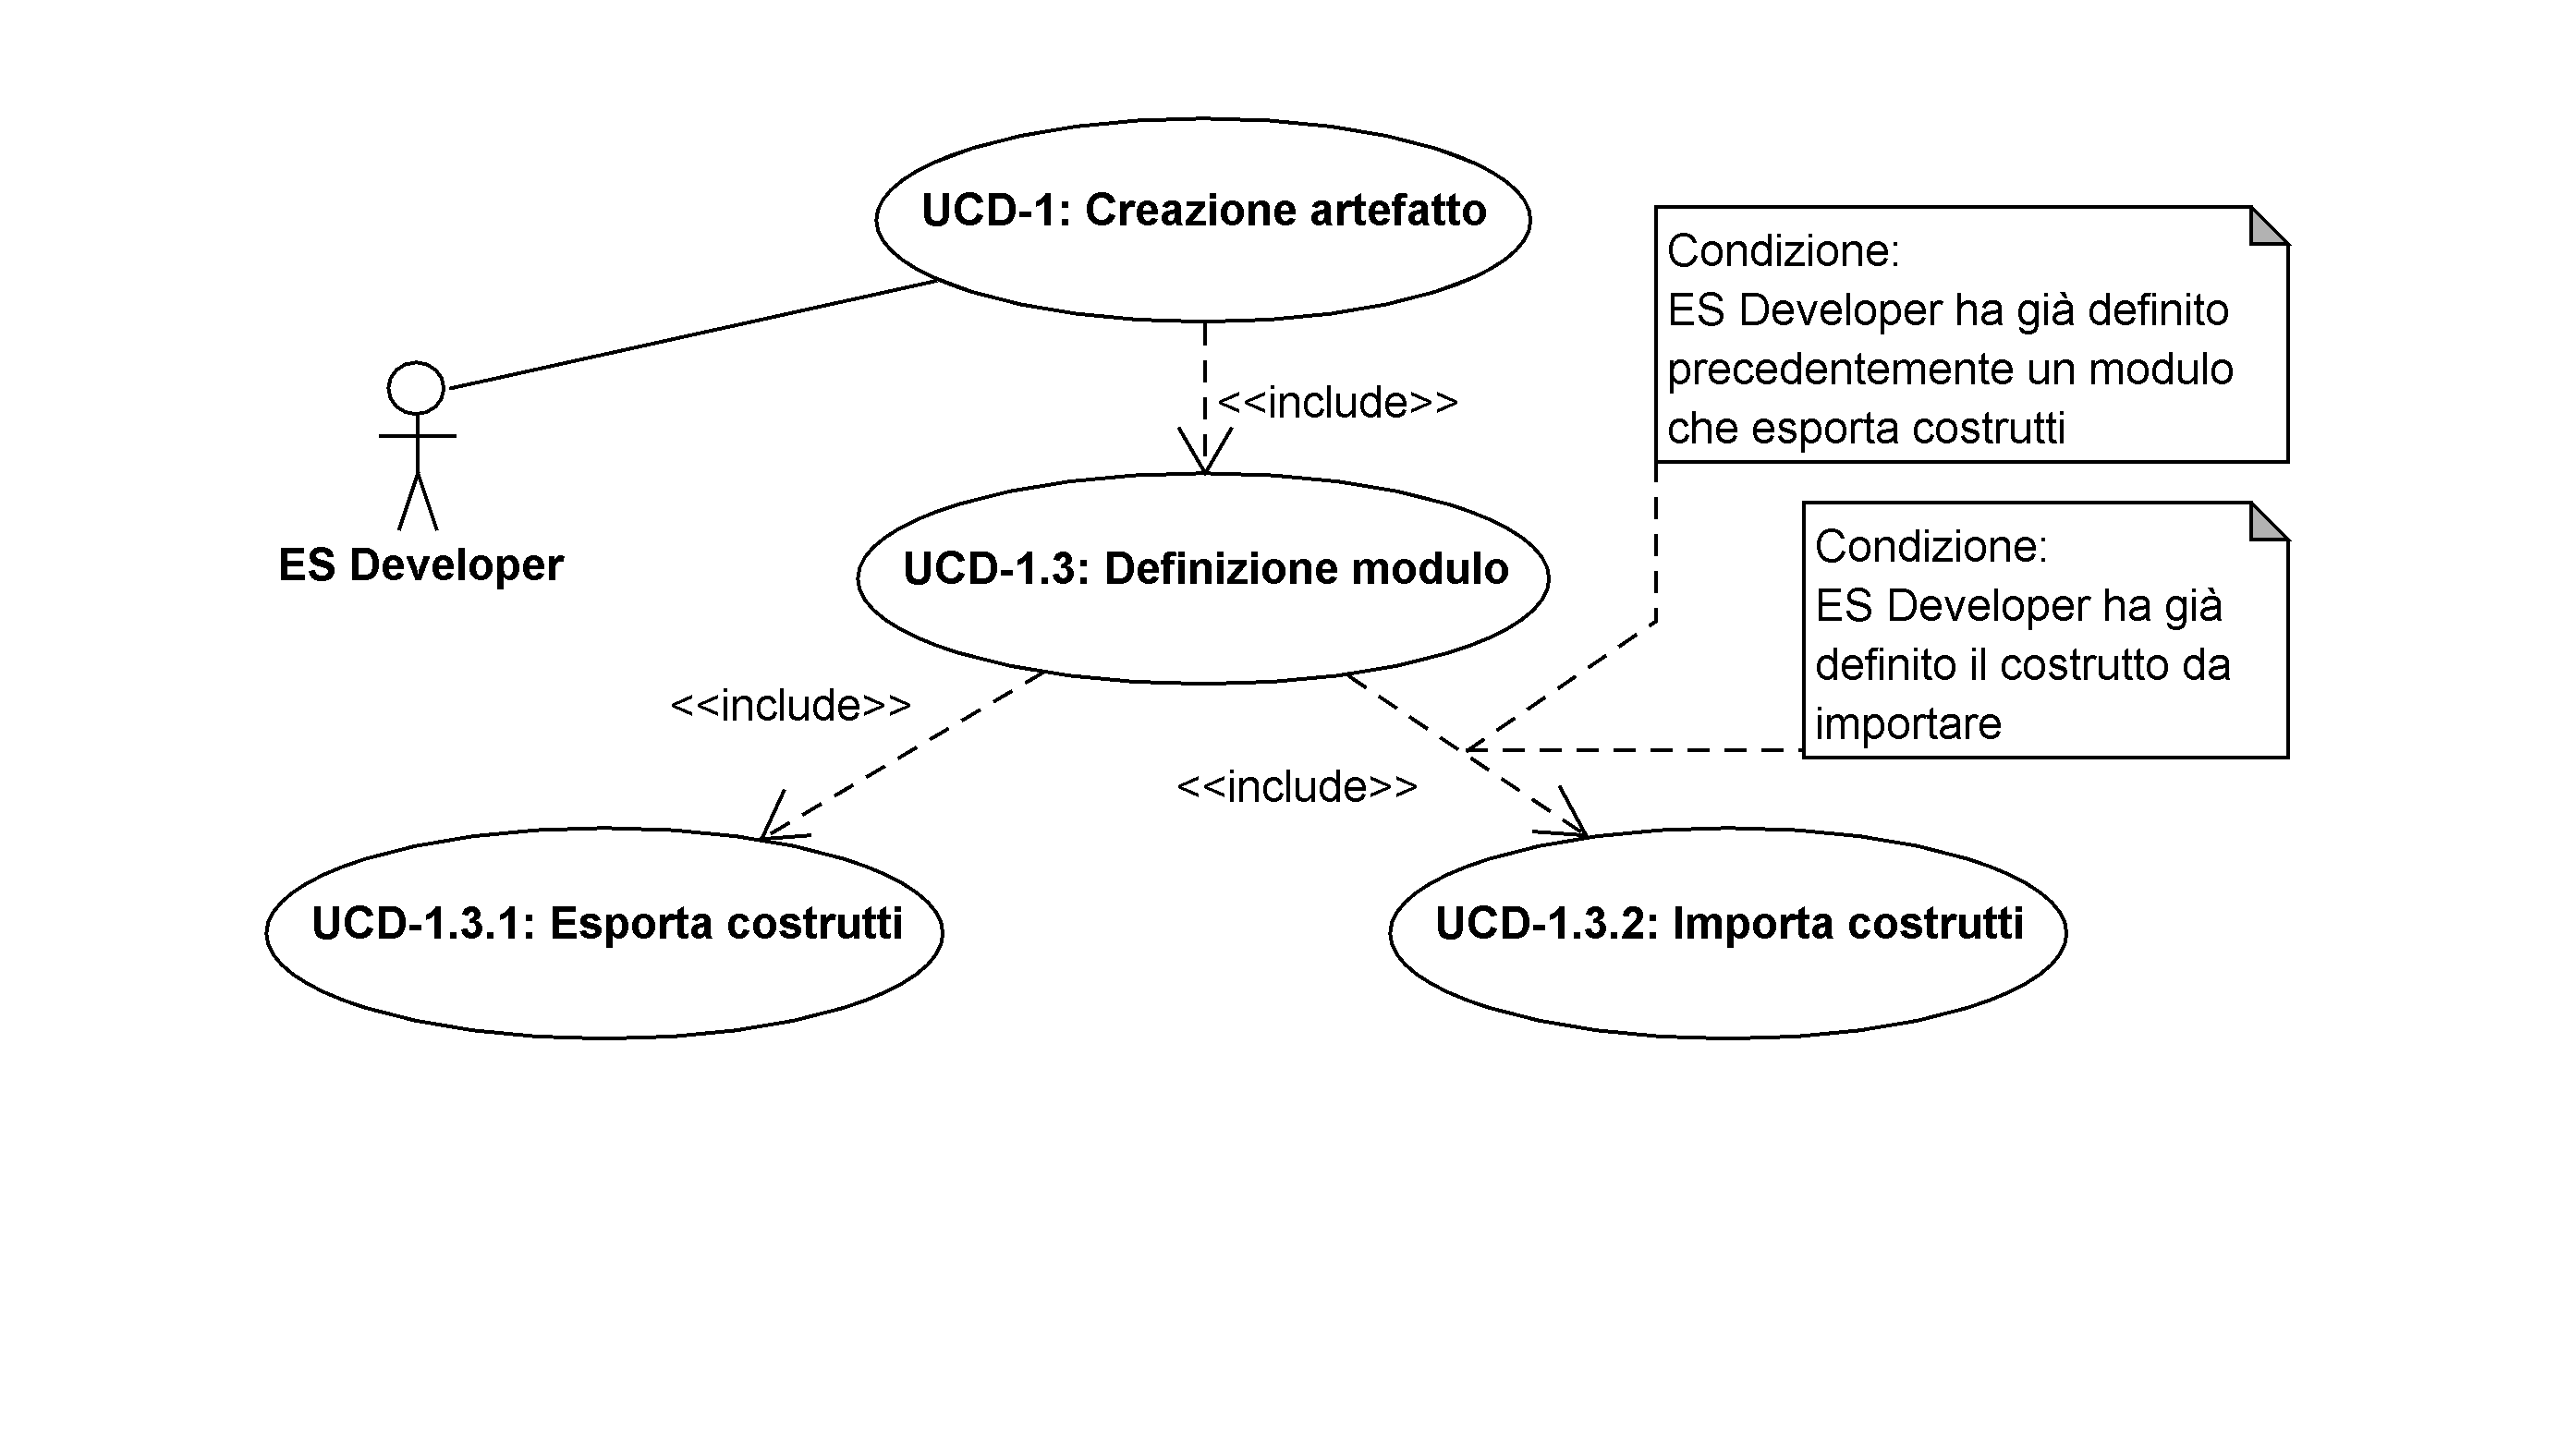
\includegraphics[width=1\textwidth]{Immagini/Capitolo2/UseCases/UCD-1_3.png}
\caption{Diagramma dei casi d'uso UCD-1.3}\label{fig:uc-ucd-1.3}
\end{figure}

\begin{itemize}
	\item \textbf{Attori:} ES Consumer
	\item \textbf{Scopo e descrizione:} l'ES Consumer deve poter eseguire un artefatto caricato nel sistema. Se l'interazione lo richiede, l'ES Consumer deve essere in grado di fornire informazioni aggiuntive, osservare l'accadimento di un evento e osservare l'output fornito dal sistema
	\item \textbf{Pre-condizioni:} il software ha correttamente caricato un artefatto ed attende istruzioni.
	\item \textbf{Post-condizioni:} il software ha correttamente eseguito le operazioni previste dall'artefatto.
	\item \textbf{Flusso principale degli eventi:}
		\begin{enumerate}
			\item l'ES Consumer richiede l'esecuzione di un artefatto
			\item il sistema esegue le operazioni previste dall'artefatto (si vedano i casi d'uso \emph{UCC-1.2.1}, \emph{UCC-1.2.3})
			\item il sistema fornisce all'ES Consumer i risultati dell'esecuzione		
		\end{enumerate}
	\item \textbf{Flusso alternativo:} 
		\begin{enumerate}
			\setcounter{enumi}{1}
			\item se un'operazione specificata nell'artefatto genera errori, il sistema notifica l'errore all'ES Consumer fornendo informazioni sulla natura del problema.
			\item il sistema ritorna nello stato iniziale
		\end{enumerate}
\end{itemize}

\subparagraph{UCD-1.3.1: Esporta costrutti}

\begin{itemize}
	\item \textbf{Attori:} ES Consumer
	\item \textbf{Scopo e descrizione:} l'ES Consumer fornisce informazioni aggiuntive 
	\item \textbf{Pre-condizioni:} il sistema richiede informazioni aggiuntive per completare l'esecuzione di un artefatto
	\item \textbf{Post-condizioni:} il sistema prosegue l'esecuzione
	\item \textbf{Flusso principale degli eventi:}
		\begin{enumerate}
			\item il sistema richiede informazioni aggiuntive
			\item l'ES Consumer fornisce le informazioni nelle forme previste dall'artefatto
			\item il sistema valuta le informazioni fornite
			\item il sistema elabora le informazioni fornite
		\end{enumerate}
	\item \textbf{Flusso alternativo:} 
		\begin{enumerate}
			\setcounter{enumi}{2}
			\item il sistema notifica l'invalidità delle informazioni fornite
			\item il flusso riprende dal punto 1 del flusso principale
		\end{enumerate}
\end{itemize}


\subparagraph{UCD-1.3.2: Importa costrutti}

\begin{itemize}
	\item \textbf{Attori:} ES Consumer
	\item \textbf{Scopo e descrizione:} l'ES Consumer deve essere in grado di valutare l'output fornito dal sistema al termine di un'operazione
	\item \textbf{Pre-condizioni:} il sistema è pronto ad esegue un'operazione
	\item \textbf{Post-condizioni:} il sistema è pronto ad eseguire una nuova operazione
	\item \textbf{Flusso principale degli eventi:}
		\begin{enumerate}
			\item il sistema esegue un'operazione
			\item il sistema fornisce una visualizzazione del risultato
			\item l'ES Consumer valuta il risultato
		\end{enumerate}
\end{itemize}



\paragraph{UCD-1.4: Definizione fatti} % nome del caso d'uso Gruppo

\begin{itemize}
	\item \textbf{Attori:} 
	\item \textbf{Scopo e descrizione:} 
	\item \textbf{Pre-condizioni:} 
	\item \textbf{Post-condizioni:} 
	\item \textbf{Flusso principale degli eventi:}
		\begin{enumerate}
			\item 
		\end{enumerate}
	\item \textbf{Flusso alternativo:} 
\end{itemize}


\paragraph{UCD-1.5: Definizione variabile globale} % nome del caso d'uso Gruppo

\begin{itemize}
	\item \textbf{Attori:} 
	\item \textbf{Scopo e descrizione:} 
	\item \textbf{Pre-condizioni:} 
	\item \textbf{Post-condizioni:} 
	\item \textbf{Flusso principale degli eventi:}
		\begin{enumerate}
			\item 
		\end{enumerate}
	\item \textbf{Flusso alternativo:} 
\end{itemize}

\paragraph{UCD-1.6: Definizione funzione} % nome del caso d'uso Gruppo

\begin{itemize}
	\item \textbf{Attori:} 
	\item \textbf{Scopo e descrizione:} 
	\item \textbf{Pre-condizioni:} 
	\item \textbf{Post-condizioni:} 
	\item \textbf{Flusso principale degli eventi:}
		\begin{enumerate}
			\item 
		\end{enumerate}
	\item \textbf{Flusso alternativo:} 
\end{itemize}
